%first chapter
\chapter{Software}
\pagenumbering{arabic} 
\thispagestyle{fancy}
GitHub: {\url{https://github.com/tobiasfalk/Assortment\_System\_Server.git}}\newline\newline
Here we describe the software design and method of saving the information about the different parts.

\section{Design Structure}

\begin{figure}[h]
	\centering
	\resizebox{\columnwidth}{!}{%
	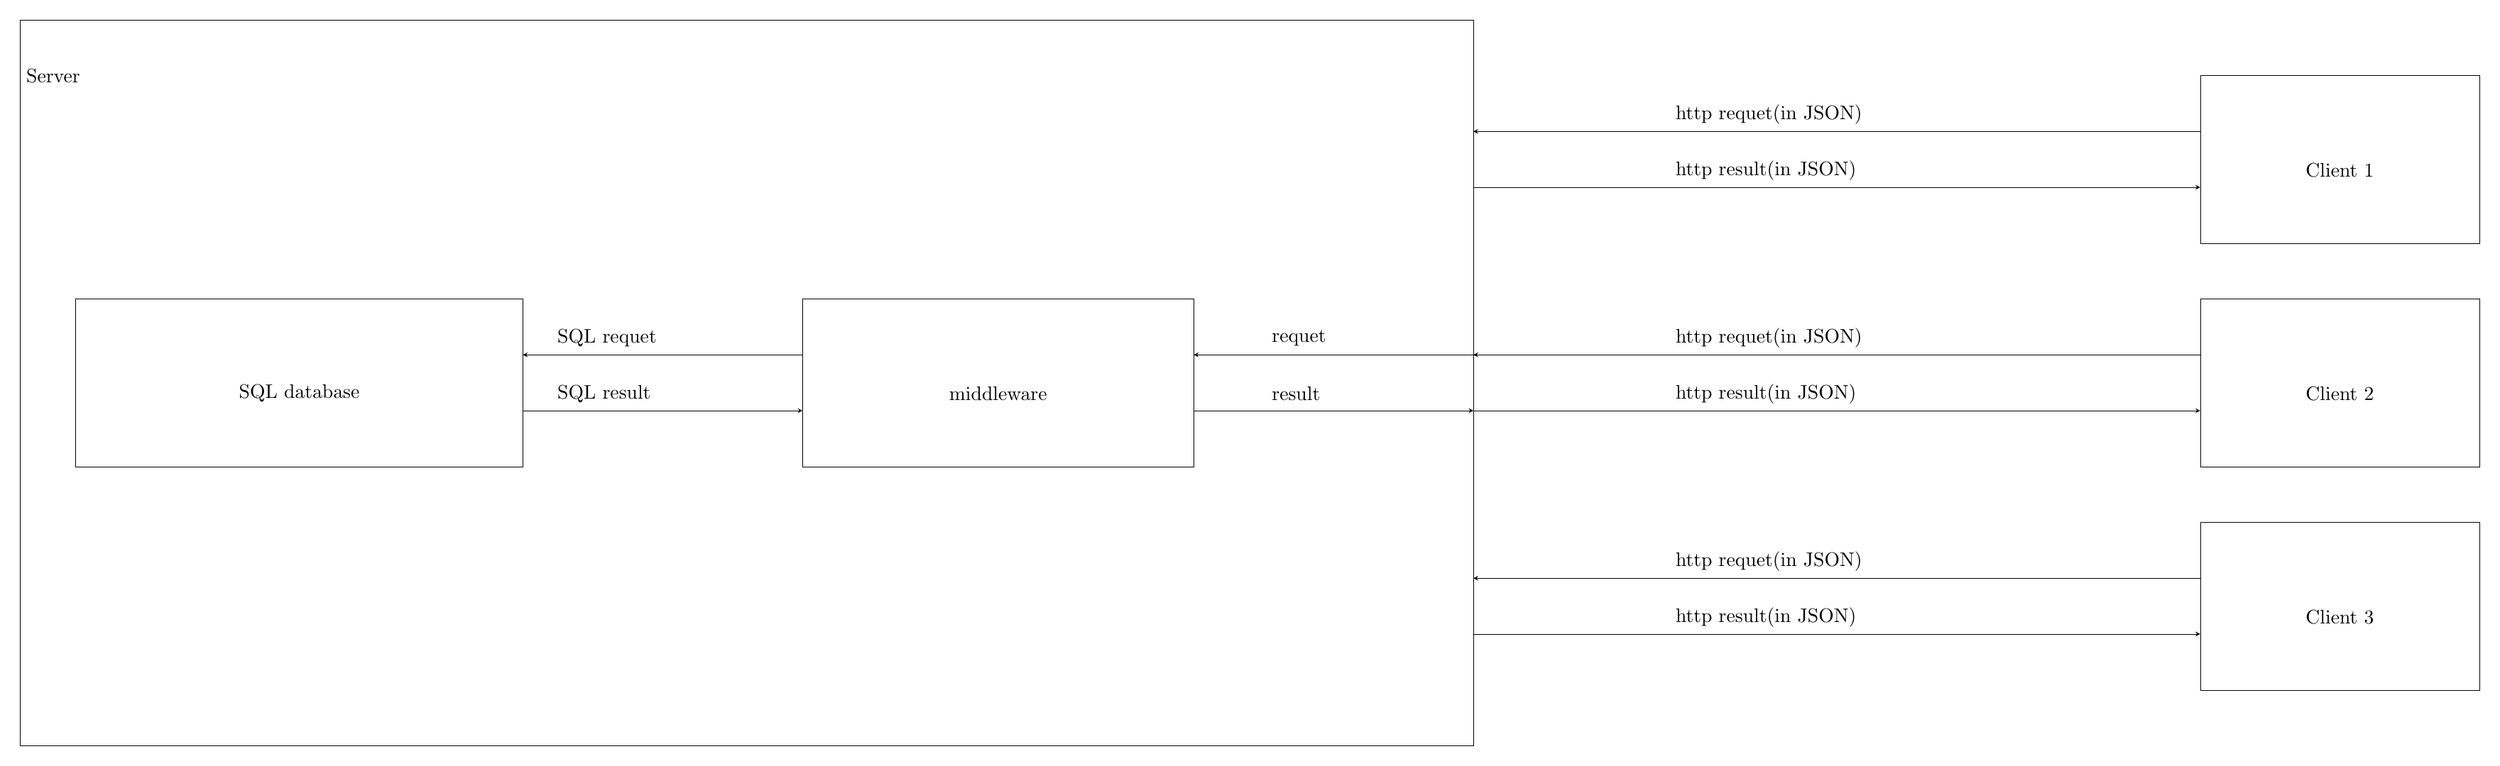
\begin{tikzpicture}
		\pgftransformxscale{1.000000}
		\pgftransformyscale{-1.000000}
		\definecolor{dialinecolor}{rgb}{0.000000, 0.000000, 0.000000}
		\pgfsetstrokecolor{dialinecolor}
		\definecolor{dialinecolor}{rgb}{1.000000, 1.000000, 1.000000}
		\pgfsetfillcolor{dialinecolor}
		\definecolor{dialinecolor}{rgb}{1.000000, 1.000000, 1.000000}
		\pgfsetfillcolor{dialinecolor}
		\fill (17.000000\du,7.000000\du)--(17.000000\du,20.000000\du)--(43.000000\du,20.000000\du)--(43.000000\du,7.000000\du)--cycle;
		\pgfsetlinewidth{0.100000\du}
		\pgfsetdash{}{0pt}
		\pgfsetdash{}{0pt}
		\pgfsetmiterjoin
		\definecolor{dialinecolor}{rgb}{0.000000, 0.000000, 0.000000}
		\pgfsetstrokecolor{dialinecolor}
		\draw (17.000000\du,7.000000\du)--(17.000000\du,20.000000\du)--(43.000000\du,20.000000\du)--(43.000000\du,7.000000\du)--cycle;
		% setfont left to latex
		\definecolor{dialinecolor}{rgb}{0.000000, 0.000000, 0.000000}
		\pgfsetstrokecolor{dialinecolor}
		\node at (30.000000\du,13.695000\du){};
		% setfont left to latex
		\definecolor{dialinecolor}{rgb}{0.000000, 0.000000, 0.000000}
		\pgfsetstrokecolor{dialinecolor}
		\node[anchor=west] at (17.000000\du,8.000000\du){Server};
		\pgfsetlinewidth{0.100000\du}
		\pgfsetdash{}{0pt}
		\pgfsetdash{}{0pt}
		\pgfsetbuttcap
		{
			\definecolor{dialinecolor}{rgb}{0.000000, 0.000000, 0.000000}
			\pgfsetfillcolor{dialinecolor}
			% was here!!!
			\pgfsetarrowsend{stealth}
			\definecolor{dialinecolor}{rgb}{0.000000, 0.000000, 0.000000}
			\pgfsetstrokecolor{dialinecolor}
			\draw (56.000000\du,9.000000\du)--(43.000000\du,9.000000\du);
		}
		\pgfsetlinewidth{0.100000\du}
		\pgfsetdash{}{0pt}
		\pgfsetdash{}{0pt}
		\pgfsetbuttcap
		{
			\definecolor{dialinecolor}{rgb}{0.000000, 0.000000, 0.000000}
			\pgfsetfillcolor{dialinecolor}
			% was here!!!
			\pgfsetarrowsend{stealth}
			\definecolor{dialinecolor}{rgb}{0.000000, 0.000000, 0.000000}
			\pgfsetstrokecolor{dialinecolor}
			\draw (43.000000\du,10.000000\du)--(56.000000\du,10.000000\du);
		}
		% setfont left to latex
		\definecolor{dialinecolor}{rgb}{0.000000, 0.000000, 0.000000}
		\pgfsetstrokecolor{dialinecolor}
		\node[anchor=west] at (46.500000\du,8.700000\du){http requet(in JSON)};
		% setfont left to latex
		\definecolor{dialinecolor}{rgb}{0.000000, 0.000000, 0.000000}
		\pgfsetstrokecolor{dialinecolor}
		\node[anchor=west] at (46.500000\du,9.700000\du){http result(in JSON)};
		\pgfsetlinewidth{0.100000\du}
		\pgfsetdash{}{0pt}
		\pgfsetdash{}{0pt}
		\pgfsetbuttcap
		{
			\definecolor{dialinecolor}{rgb}{0.000000, 0.000000, 0.000000}
			\pgfsetfillcolor{dialinecolor}
			% was here!!!
			\pgfsetarrowsend{stealth}
			\definecolor{dialinecolor}{rgb}{0.000000, 0.000000, 0.000000}
			\pgfsetstrokecolor{dialinecolor}
			\draw (56.000000\du,13.000000\du)--(43.000000\du,13.000000\du);
		}
		\pgfsetlinewidth{0.100000\du}
		\pgfsetdash{}{0pt}
		\pgfsetdash{}{0pt}
		\pgfsetbuttcap
		{
			\definecolor{dialinecolor}{rgb}{0.000000, 0.000000, 0.000000}
			\pgfsetfillcolor{dialinecolor}
			% was here!!!
			\pgfsetarrowsend{stealth}
			\definecolor{dialinecolor}{rgb}{0.000000, 0.000000, 0.000000}
			\pgfsetstrokecolor{dialinecolor}
			\draw (43.000000\du,14.000000\du)--(56.000000\du,14.000000\du);
		}
		% setfont left to latex
		\definecolor{dialinecolor}{rgb}{0.000000, 0.000000, 0.000000}
		\pgfsetstrokecolor{dialinecolor}
		\node[anchor=west] at (46.500000\du,12.700000\du){http requet(in JSON)};
		% setfont left to latex
		\definecolor{dialinecolor}{rgb}{0.000000, 0.000000, 0.000000}
		\pgfsetstrokecolor{dialinecolor}
		\node[anchor=west] at (46.500000\du,13.700000\du){http result(in JSON)};
		\pgfsetlinewidth{0.100000\du}
		\pgfsetdash{}{0pt}
		\pgfsetdash{}{0pt}
		\pgfsetbuttcap
		{
			\definecolor{dialinecolor}{rgb}{0.000000, 0.000000, 0.000000}
			\pgfsetfillcolor{dialinecolor}
			% was here!!!
			\pgfsetarrowsend{stealth}
			\definecolor{dialinecolor}{rgb}{0.000000, 0.000000, 0.000000}
			\pgfsetstrokecolor{dialinecolor}
			\draw (56.000000\du,17.000000\du)--(43.000000\du,17.000000\du);
		}
		\pgfsetlinewidth{0.100000\du}
		\pgfsetdash{}{0pt}
		\pgfsetdash{}{0pt}
		\pgfsetbuttcap
		{
			\definecolor{dialinecolor}{rgb}{0.000000, 0.000000, 0.000000}
			\pgfsetfillcolor{dialinecolor}
			% was here!!!
			\pgfsetarrowsend{stealth}
			\definecolor{dialinecolor}{rgb}{0.000000, 0.000000, 0.000000}
			\pgfsetstrokecolor{dialinecolor}
			\draw (43.000000\du,18.000000\du)--(56.000000\du,18.000000\du);
		}
		% setfont left to latex
		\definecolor{dialinecolor}{rgb}{0.000000, 0.000000, 0.000000}
		\pgfsetstrokecolor{dialinecolor}
		\node[anchor=west] at (46.500000\du,16.700000\du){http requet(in JSON)};
		% setfont left to latex
		\definecolor{dialinecolor}{rgb}{0.000000, 0.000000, 0.000000}
		\pgfsetstrokecolor{dialinecolor}
		\node[anchor=west] at (46.500000\du,17.700000\du){http result(in JSON)};
		\pgfsetlinewidth{0.100000\du}
		\pgfsetdash{}{0pt}
		\pgfsetdash{}{0pt}
		\pgfsetbuttcap
		{
			\definecolor{dialinecolor}{rgb}{0.000000, 0.000000, 0.000000}
			\pgfsetfillcolor{dialinecolor}
			% was here!!!
			\pgfsetarrowsend{stealth}
			\definecolor{dialinecolor}{rgb}{0.000000, 0.000000, 0.000000}
			\pgfsetstrokecolor{dialinecolor}
			\draw (43.000000\du,13.000000\du)--(38.000000\du,13.000000\du);
		}
		\pgfsetlinewidth{0.100000\du}
		\pgfsetdash{}{0pt}
		\pgfsetdash{}{0pt}
		\pgfsetbuttcap
		{
			\definecolor{dialinecolor}{rgb}{0.000000, 0.000000, 0.000000}
			\pgfsetfillcolor{dialinecolor}
			% was here!!!
			\pgfsetarrowsend{stealth}
			\definecolor{dialinecolor}{rgb}{0.000000, 0.000000, 0.000000}
			\pgfsetstrokecolor{dialinecolor}
			\draw (38.000000\du,14.000000\du)--(43.000000\du,14.000000\du);
		}
		% setfont left to latex
		\definecolor{dialinecolor}{rgb}{0.000000, 0.000000, 0.000000}
		\pgfsetstrokecolor{dialinecolor}
		\node[anchor=west] at (39.279100\du,12.696000\du){requet};
		% setfont left to latex
		\definecolor{dialinecolor}{rgb}{0.000000, 0.000000, 0.000000}
		\pgfsetstrokecolor{dialinecolor}
		\node[anchor=west] at (39.279100\du,13.700000\du){result};
		\pgfsetlinewidth{0.100000\du}
		\pgfsetdash{}{0pt}
		\pgfsetdash{}{0pt}
		\pgfsetbuttcap
		{
			\definecolor{dialinecolor}{rgb}{0.000000, 0.000000, 0.000000}
			\pgfsetfillcolor{dialinecolor}
			% was here!!!
			\pgfsetarrowsend{stealth}
			\definecolor{dialinecolor}{rgb}{0.000000, 0.000000, 0.000000}
			\pgfsetstrokecolor{dialinecolor}
			\draw (31.000000\du,13.000000\du)--(26.000000\du,13.000000\du);
		}
		\pgfsetlinewidth{0.100000\du}
		\pgfsetdash{}{0pt}
		\pgfsetdash{}{0pt}
		\pgfsetbuttcap
		{
			\definecolor{dialinecolor}{rgb}{0.000000, 0.000000, 0.000000}
			\pgfsetfillcolor{dialinecolor}
			% was here!!!
			\pgfsetarrowsend{stealth}
			\definecolor{dialinecolor}{rgb}{0.000000, 0.000000, 0.000000}
			\pgfsetstrokecolor{dialinecolor}
			\draw (26.000000\du,14.000000\du)--(31.000000\du,14.000000\du);
		}
		% setfont left to latex
		\definecolor{dialinecolor}{rgb}{0.000000, 0.000000, 0.000000}
		\pgfsetstrokecolor{dialinecolor}
		\node[anchor=west] at (26.500000\du,12.700000\du){SQL requet};
		% setfont left to latex
		\definecolor{dialinecolor}{rgb}{0.000000, 0.000000, 0.000000}
		\pgfsetstrokecolor{dialinecolor}
		\node[anchor=west] at (26.500000\du,13.70000\du){SQL result};
		\definecolor{dialinecolor}{rgb}{1.000000, 1.000000, 1.000000}
		\pgfsetfillcolor{dialinecolor}
		\fill (56.000000\du,8.000000\du)--(56.000000\du,11.000000\du)--(61.000000\du,11.000000\du)--(61.000000\du,8.000000\du)--cycle;
		\pgfsetlinewidth{0.100000\du}
		\pgfsetdash{}{0pt}
		\pgfsetdash{}{0pt}
		\pgfsetmiterjoin
		\definecolor{dialinecolor}{rgb}{0.000000, 0.000000, 0.000000}
		\pgfsetstrokecolor{dialinecolor}
		\draw (56.000000\du,8.000000\du)--(56.000000\du,11.000000\du)--(61.000000\du,11.000000\du)--(61.000000\du,8.000000\du)--cycle;
		% setfont left to latex
		\definecolor{dialinecolor}{rgb}{0.000000, 0.000000, 0.000000}
		\pgfsetstrokecolor{dialinecolor}
		\node at (58.500000\du,9.695000\du){Client 1};
		\definecolor{dialinecolor}{rgb}{1.000000, 1.000000, 1.000000}
		\pgfsetfillcolor{dialinecolor}
		\fill (56.000000\du,12.000000\du)--(56.000000\du,15.000000\du)--(61.000000\du,15.000000\du)--(61.000000\du,12.000000\du)--cycle;
		\pgfsetlinewidth{0.100000\du}
		\pgfsetdash{}{0pt}
		\pgfsetdash{}{0pt}
		\pgfsetmiterjoin
		\definecolor{dialinecolor}{rgb}{0.000000, 0.000000, 0.000000}
		\pgfsetstrokecolor{dialinecolor}
		\draw (56.000000\du,12.000000\du)--(56.000000\du,15.000000\du)--(61.000000\du,15.000000\du)--(61.000000\du,12.000000\du)--cycle;
		% setfont left to latex
		\definecolor{dialinecolor}{rgb}{0.000000, 0.000000, 0.000000}
		\pgfsetstrokecolor{dialinecolor}
		\node at (58.500000\du,13.695000\du){Client 2};
		\definecolor{dialinecolor}{rgb}{1.000000, 1.000000, 1.000000}
		\pgfsetfillcolor{dialinecolor}
		\fill (56.000000\du,16.000000\du)--(56.000000\du,19.000000\du)--(61.000000\du,19.000000\du)--(61.000000\du,16.000000\du)--cycle;
		\pgfsetlinewidth{0.100000\du}
		\pgfsetdash{}{0pt}
		\pgfsetdash{}{0pt}
		\pgfsetmiterjoin
		\definecolor{dialinecolor}{rgb}{0.000000, 0.000000, 0.000000}
		\pgfsetstrokecolor{dialinecolor}
		\draw (56.000000\du,16.000000\du)--(56.000000\du,19.000000\du)--(61.000000\du,19.000000\du)--(61.000000\du,16.000000\du)--cycle;
		% setfont left to latex
		\definecolor{dialinecolor}{rgb}{0.000000, 0.000000, 0.000000}
		\pgfsetstrokecolor{dialinecolor}
		\node at (58.500000\du,17.695000\du){Client 3};
		\definecolor{dialinecolor}{rgb}{1.000000, 1.000000, 1.000000}
		\pgfsetfillcolor{dialinecolor}
		\fill (31.000000\du,12.000000\du)--(31.000000\du,15.000000\du)--(38.000000\du,15.000000\du)--(38.000000\du,12.000000\du)--cycle;
		\pgfsetlinewidth{0.100000\du}
		\pgfsetdash{}{0pt}
		\pgfsetdash{}{0pt}
		\pgfsetmiterjoin
		\definecolor{dialinecolor}{rgb}{0.000000, 0.000000, 0.000000}
		\pgfsetstrokecolor{dialinecolor}
		\draw (31.000000\du,12.000000\du)--(31.000000\du,15.000000\du)--(38.000000\du,15.000000\du)--(38.000000\du,12.000000\du)--cycle;
		% setfont left to latex
		\definecolor{dialinecolor}{rgb}{0.000000, 0.000000, 0.000000}
		\pgfsetstrokecolor{dialinecolor}
		\node at (34.500000\du,13.695000\du){middleware};
		\definecolor{dialinecolor}{rgb}{1.000000, 1.000000, 1.000000}
		\pgfsetfillcolor{dialinecolor}
		\fill (18.000000\du,12.000000\du)--(18.000000\du,15.000000\du)--(26.000000\du,15.000000\du)--(26.000000\du,12.000000\du)--cycle;
		\pgfsetlinewidth{0.100000\du}
		\pgfsetdash{}{0pt}
		\pgfsetdash{}{0pt}
		\pgfsetmiterjoin
		\definecolor{dialinecolor}{rgb}{0.000000, 0.000000, 0.000000}
		\pgfsetstrokecolor{dialinecolor}
		\draw (18.000000\du,12.000000\du)--(18.000000\du,15.000000\du)--(26.000000\du,15.000000\du)--(26.000000\du,12.000000\du)--cycle;
		% setfont left to latex
		\definecolor{dialinecolor}{rgb}{0.000000, 0.000000, 0.000000}
		\pgfsetstrokecolor{dialinecolor}
		\node at (22.000000\du,13.695000\du){SQL database};
	\end{tikzpicture}%
	}
	\caption{The design structure visualised}
\end{figure}
The basic idea is that we have one server where a SQL database runs and that there is an middleware that provides a REST API interface for the DB. The clients than work with this API, the client can be web based or as an Program direct on the PC or Mobile phone.

\newpage
\section{Server}
On the Server there are two things, the SQL database, where all the information is stored and the middle ware, witch provides an REST API interface for the DB.

\subsection{SQL database}
The SQL databse is a Postgessql\footnote{Postgessql webpage:{\url{https://www.postgresql.org/}}} database and is designed in an program named PgModeler\footnote{PgModeler webpage: {\url{https://pgmodeler.io/}}}. It has the main task of safeing the known information about the parts that are maneged in the system.
\newline\newline
The DB is spilt in to 6 schemas:
\begin{itemize}
	\item parts
	\item storage
	\item global
	\item assemblies
	\item vendors
	\item kicad
\end{itemize}

\newpage
\subsubsection{Schema "parts"}
In this schema you can find all the basic information about the parts. You can not find where the part is physically stored.

In the "middle" of the schema there is the $parts.parts$ table where you will find all the attributes of an part that each needs to have. That includes:
\begin{itemize}
	\item id(not set by the user)
	\item name
	\item description
	\item weight
	\item type
\end{itemize}

The 3d Model part of this schema is not yet designed.

\begin{figure}
\includegraphics[width=0.98\textheight,angle =90]{db-model_parts}
\centering
\caption{The design of the parts schema}
\end{figure}

\newpage
\subsubsection{Schema "storage"}
In this schema you can find in witch box, drawer and cabinet an part is stored. You need to know that one part can be stored at multiple places in the system. You also should know that in one cabinet there can be one ore multiple drawers and in one drawer there can be one ore multiple boxes.

\begin{figure}
	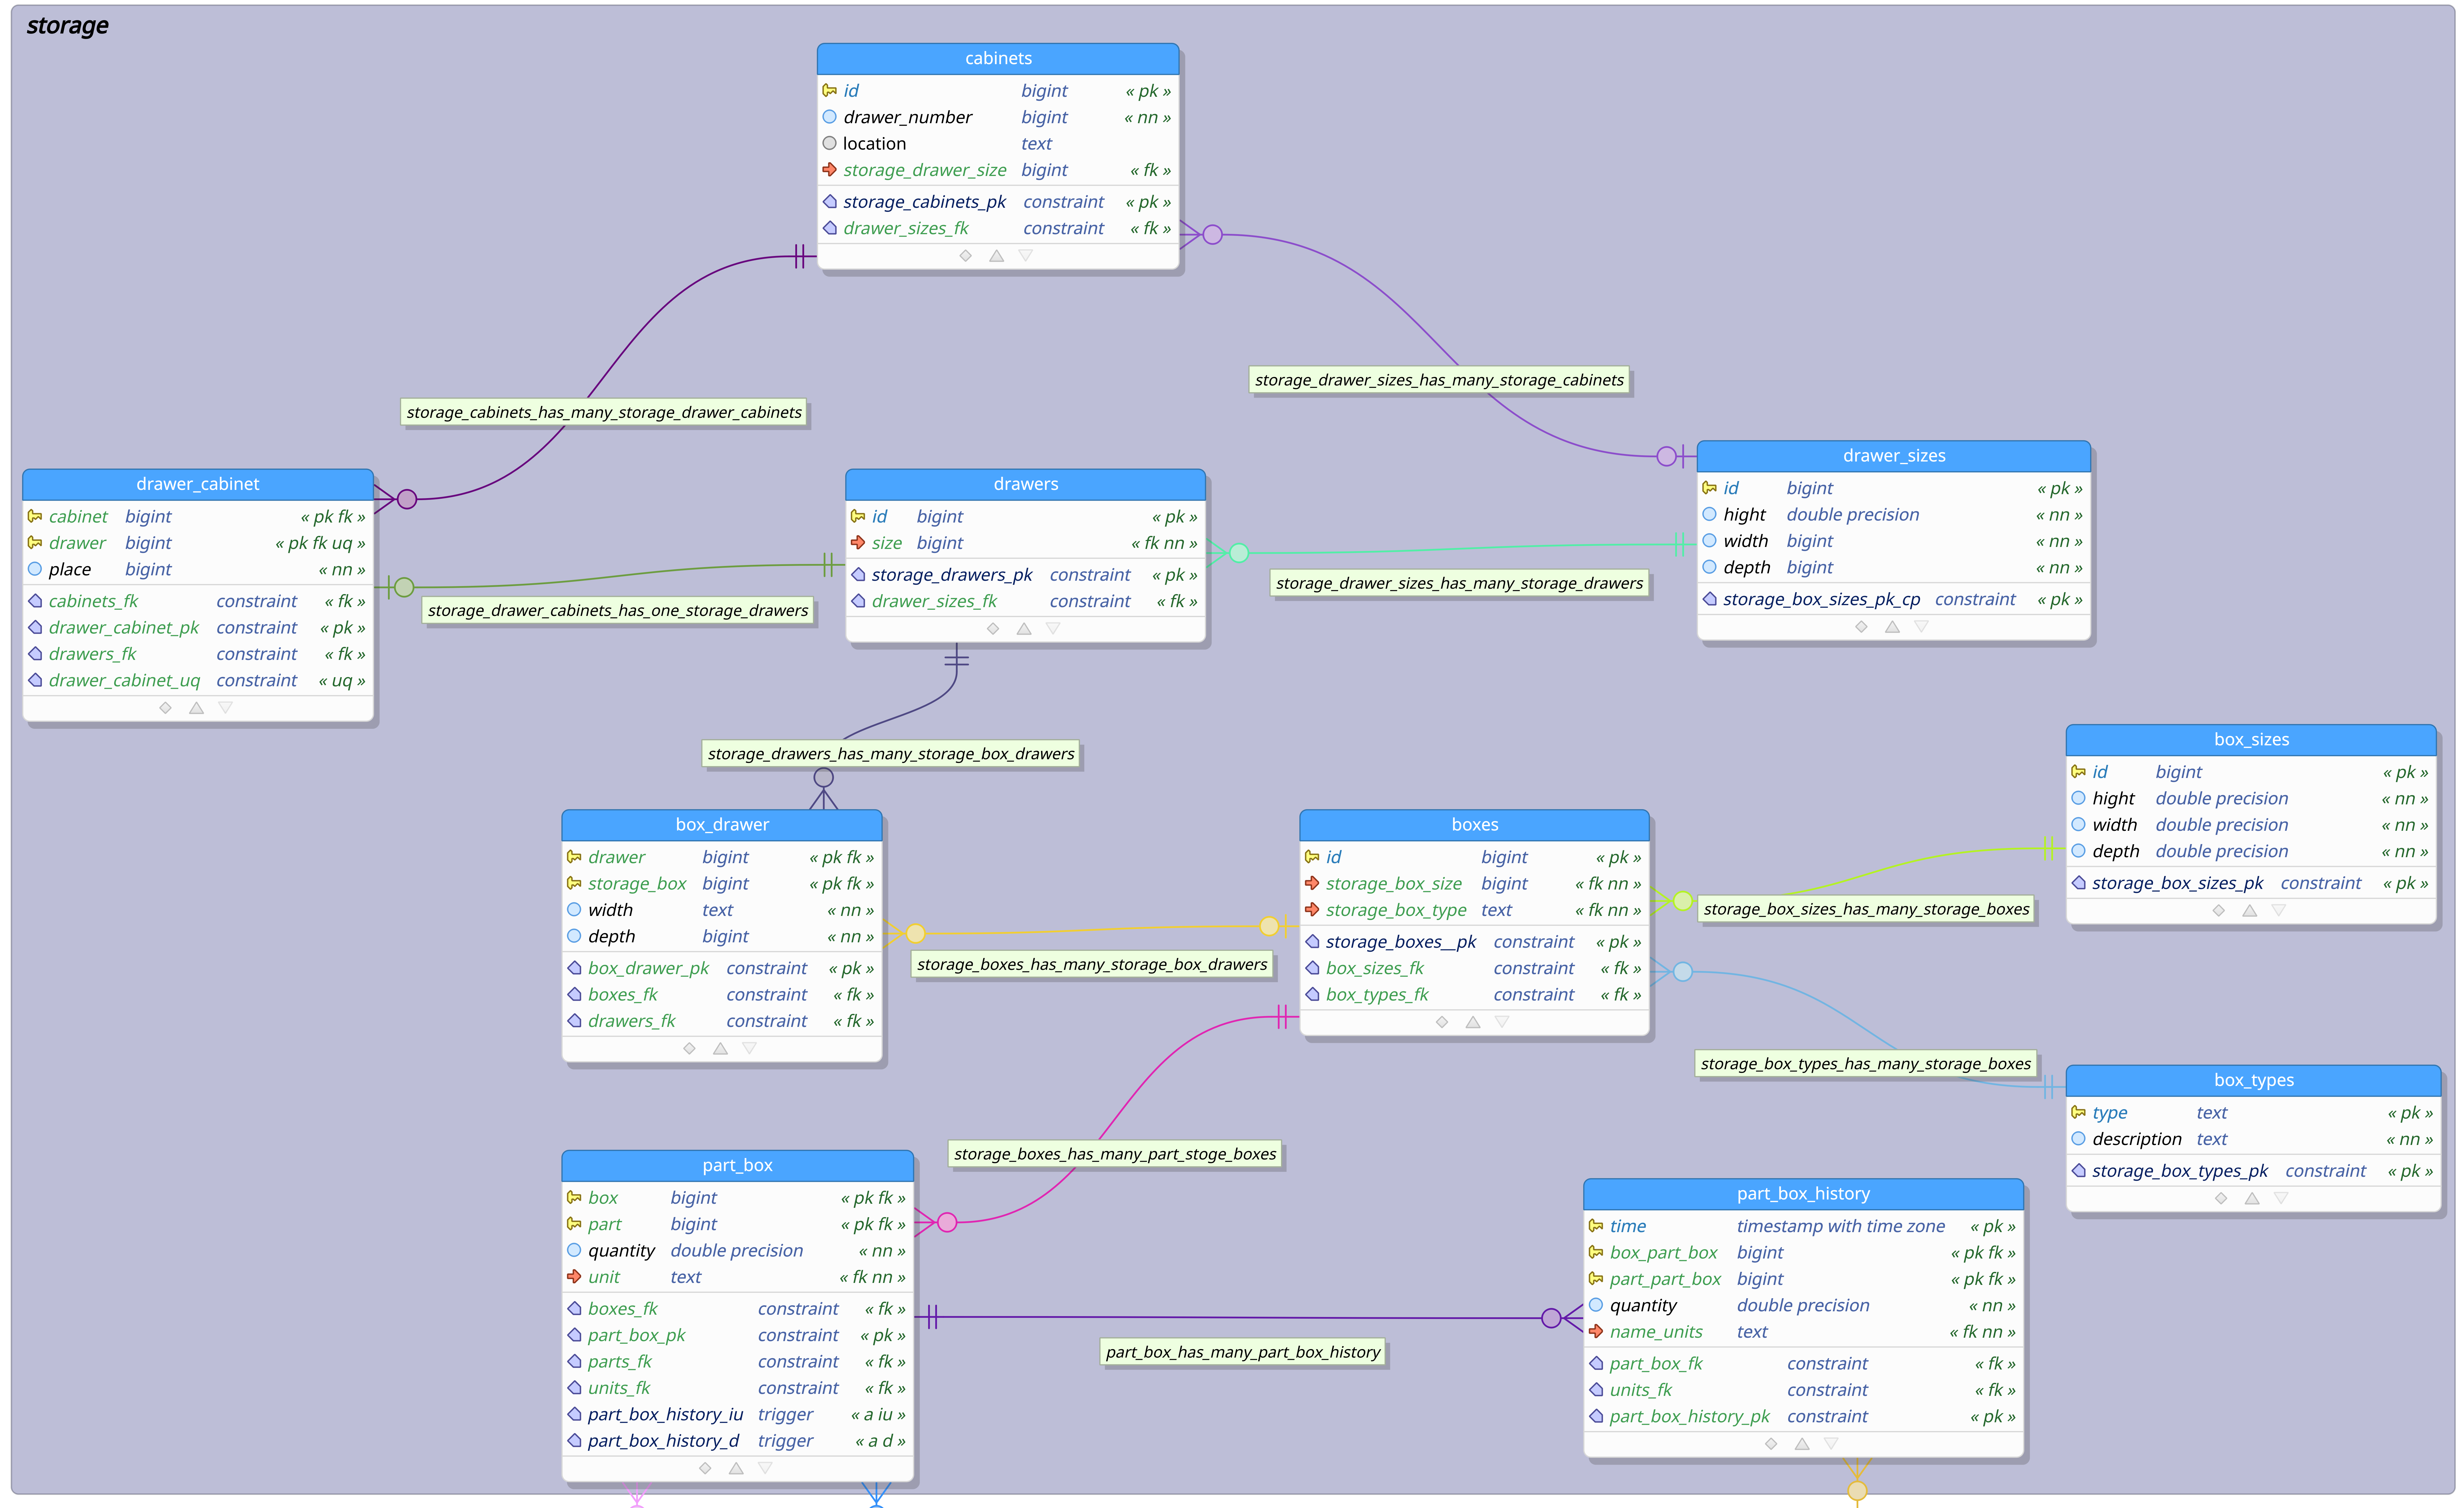
\includegraphics[width=0.98\textheight,angle =90]{db-model_storage}
	\centering
	\caption{The design of the storage schema}
\end{figure}

\newpage
\subsubsection{Schema "global"}
Here you can find all the things that are needed globally like units, currency's and file types.

\begin{figure}[h]
	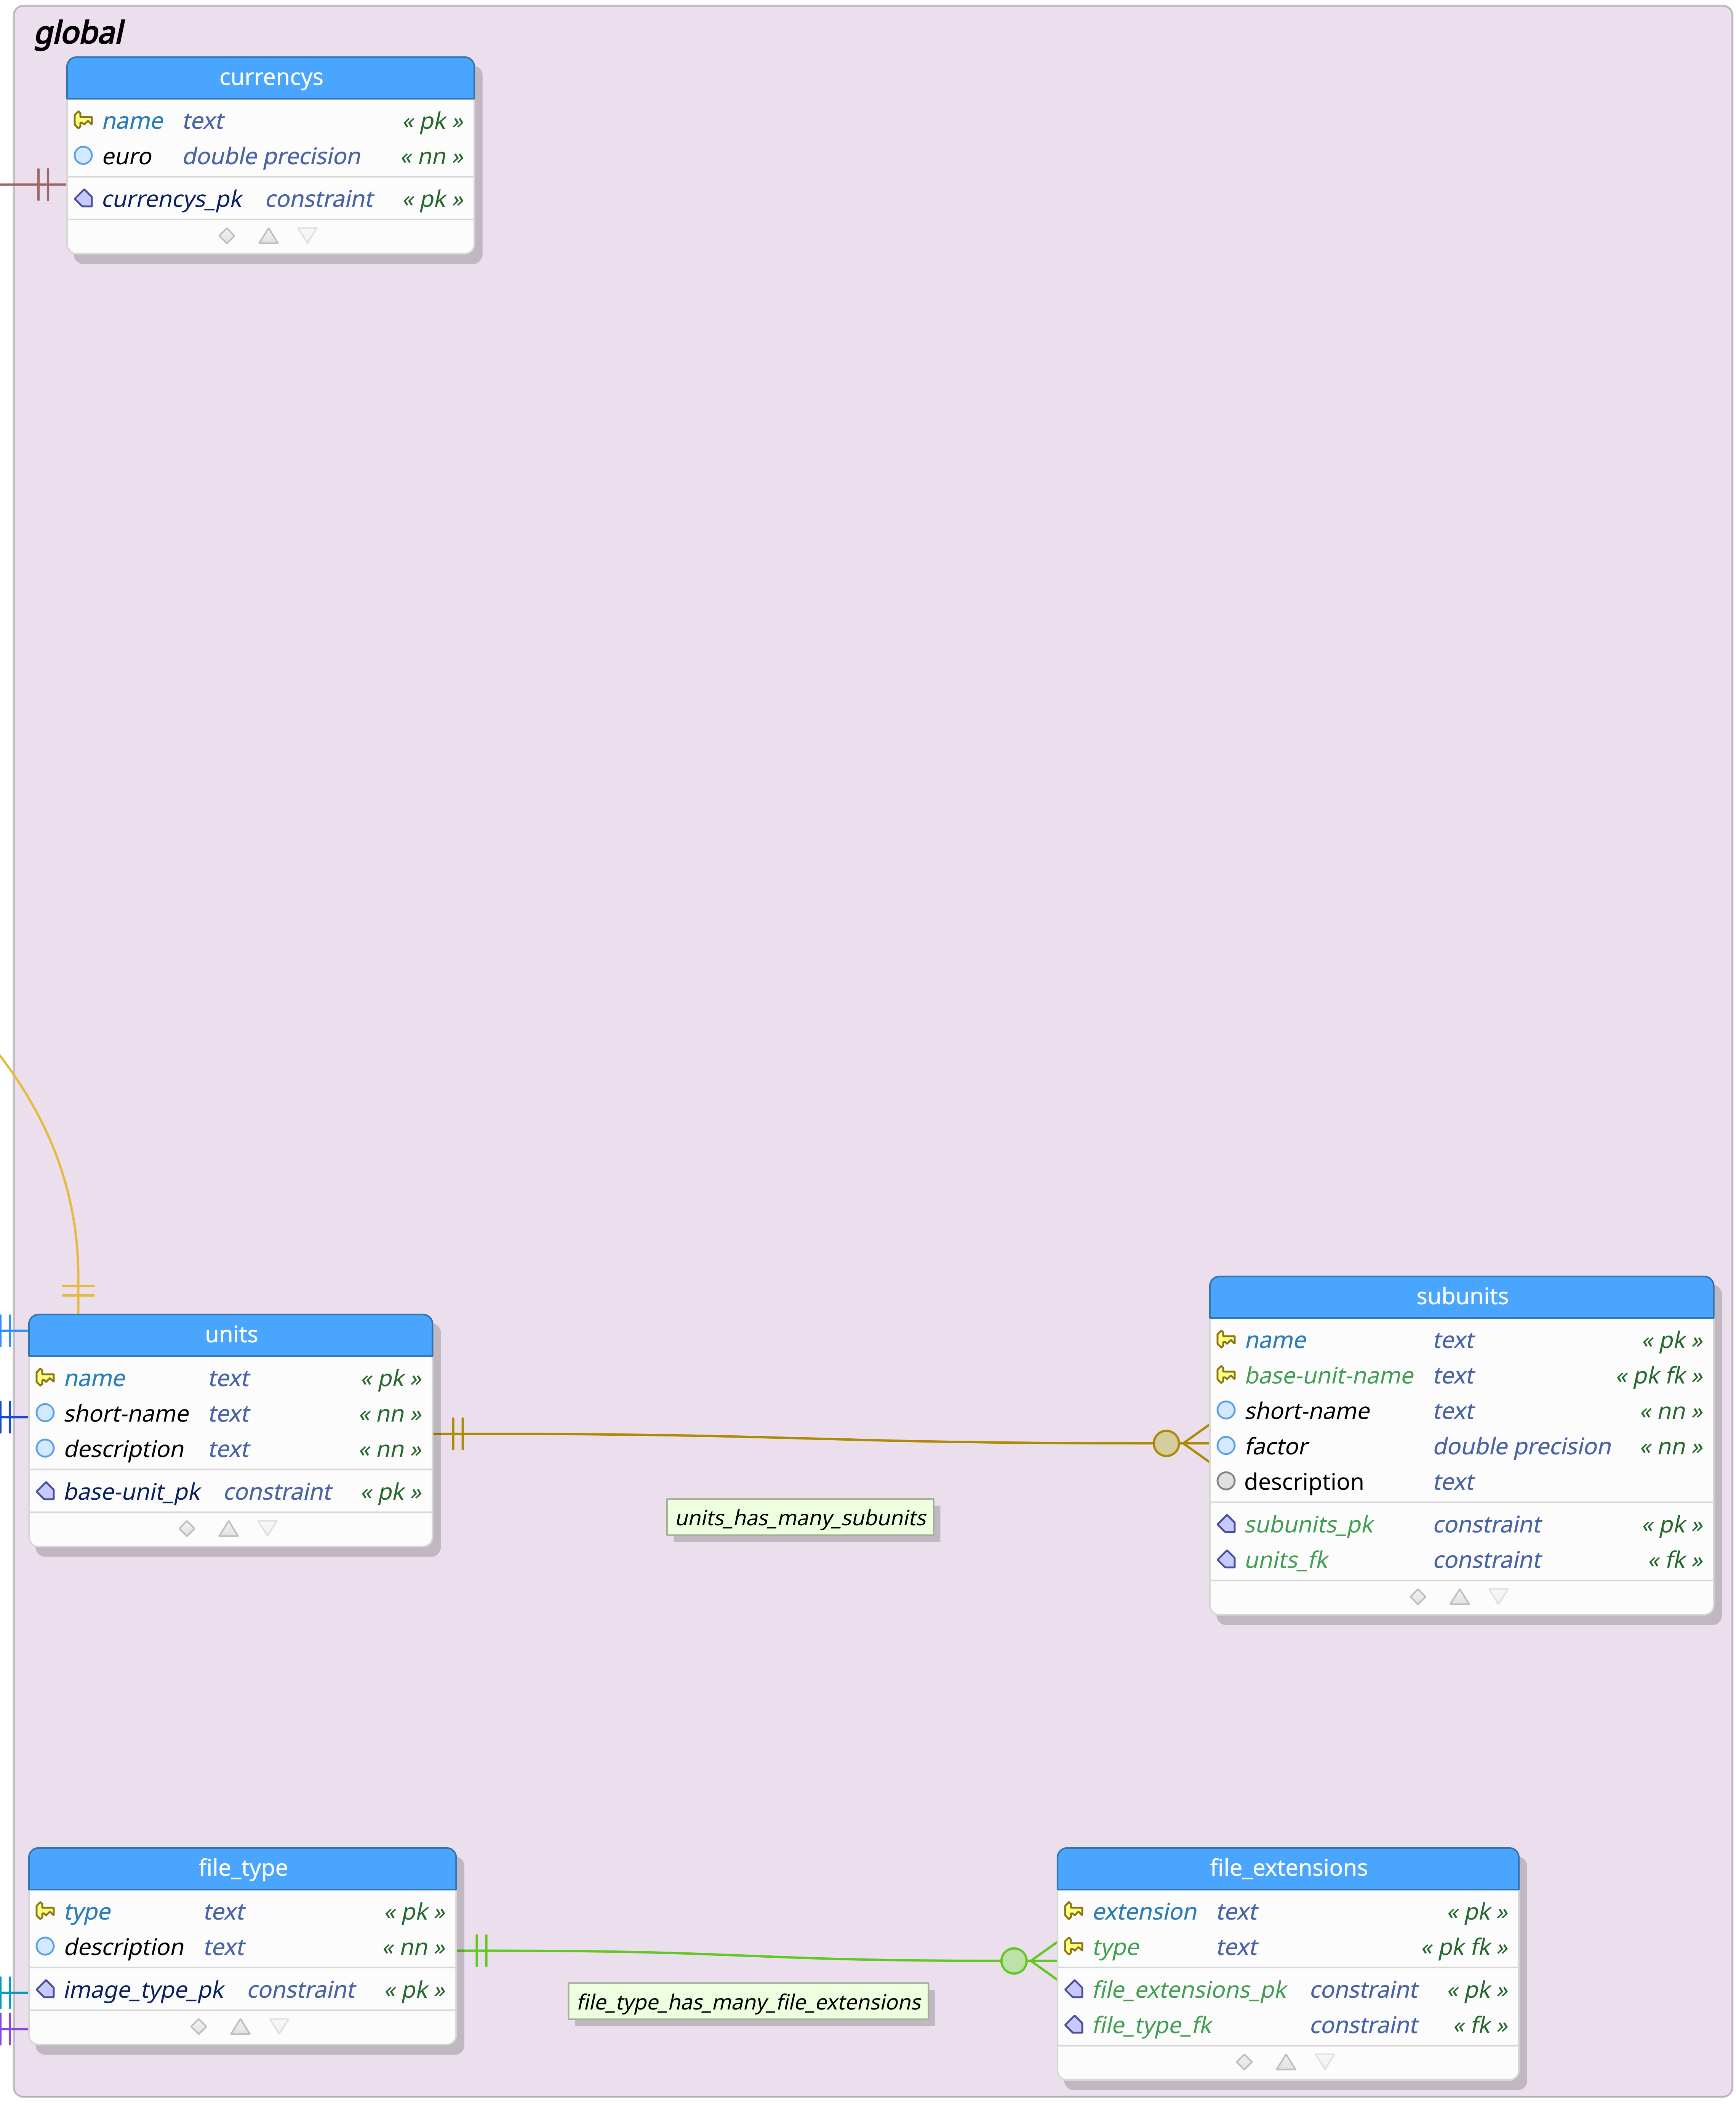
\includegraphics[width=0.8\columnwidth]{db-model_global}
	\centering
	\caption{The design of the global schema}
\end{figure}

\newpage
\subsubsection{Schema "assemblies"}
Here multiple parts are groped as assemblies to make it easier to fined all parts that go to one project.

\begin{figure}[h]
	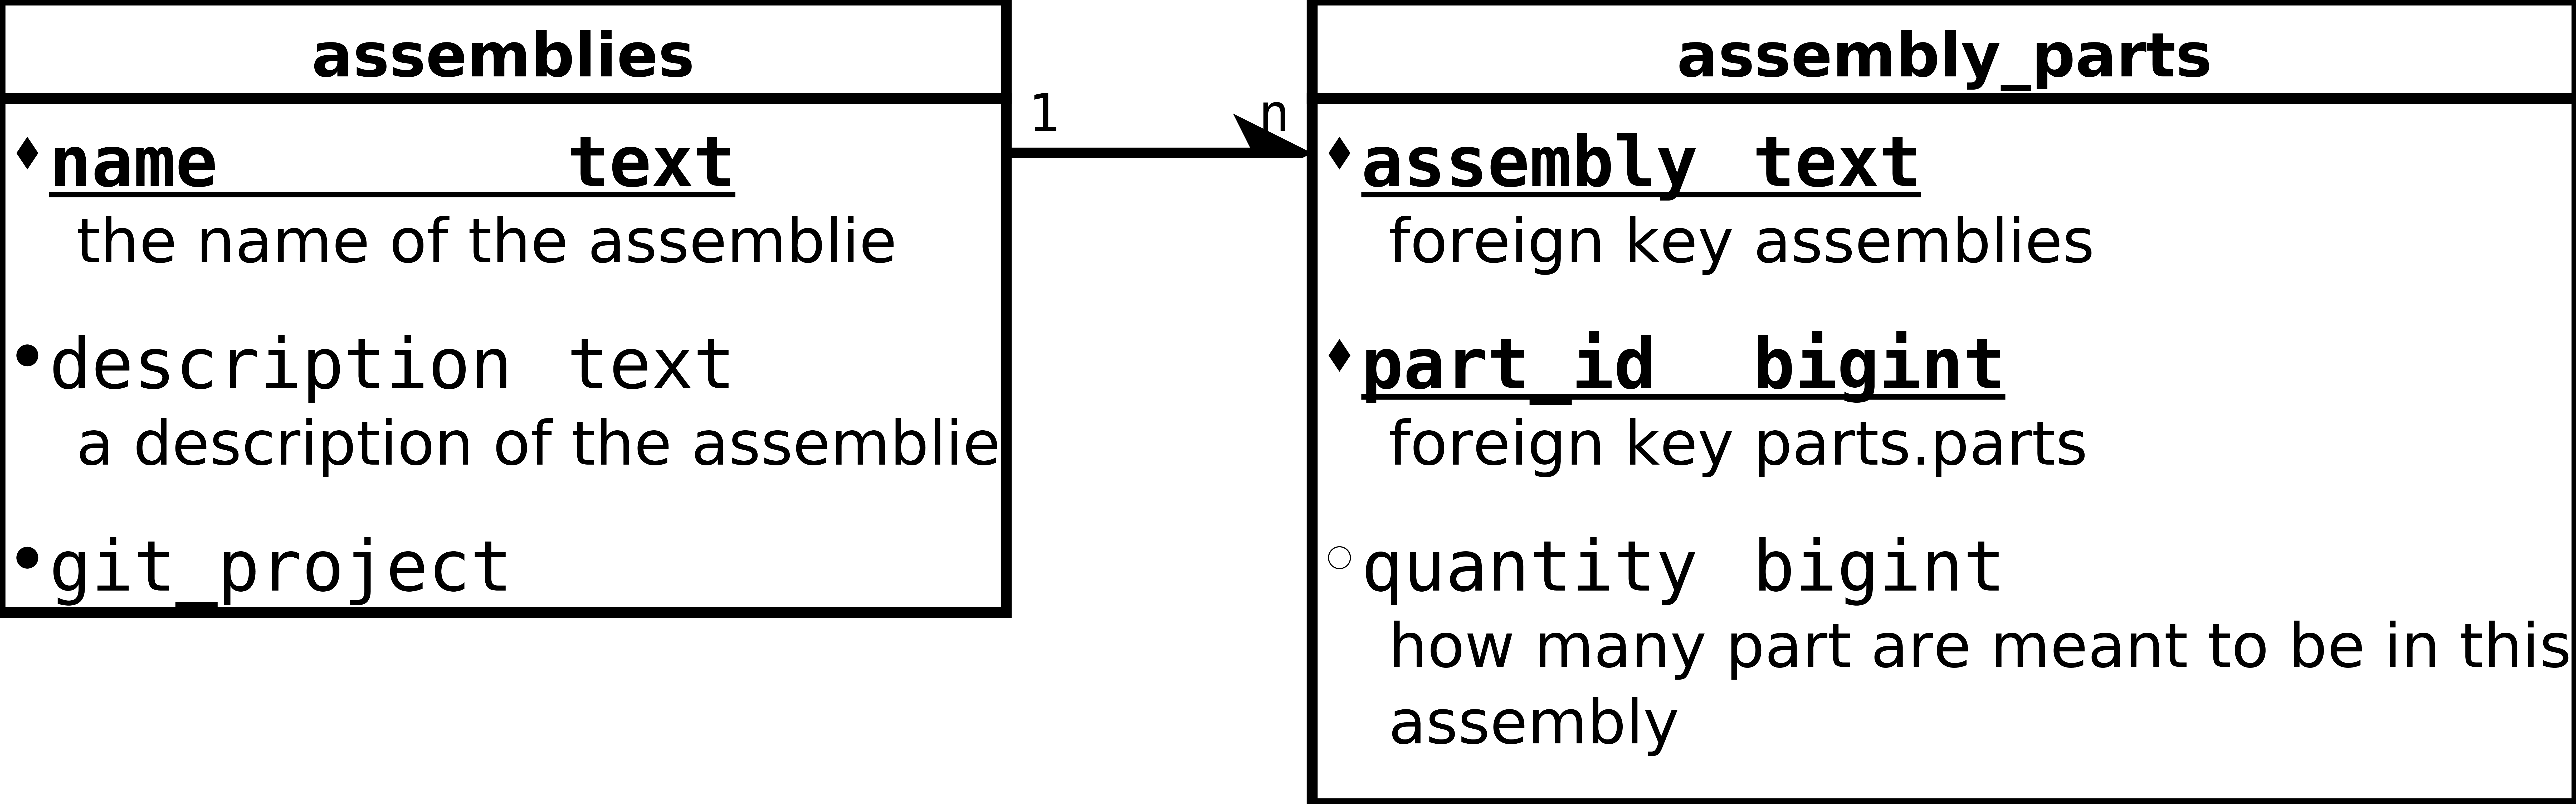
\includegraphics[width=\columnwidth]{db-model_assemblies}
	\centering
	\caption{The design of the assemblies schema}
\end{figure}

\newpage
\subsubsection{Schema "vendors"}
Here you can find all the necessary information about a vendor or manufacture.

\begin{figure}[h]
	\includegraphics[width={0.25\columnwidth}]{db-model_vendors}
	\centering
	\caption{The design of the storage schema}
\end{figure}

\newpage
\subsubsection{Schema "kicad"}
Here you can find the kicad schematic and pcb symbol for the parts.

\begin{figure}[h]
	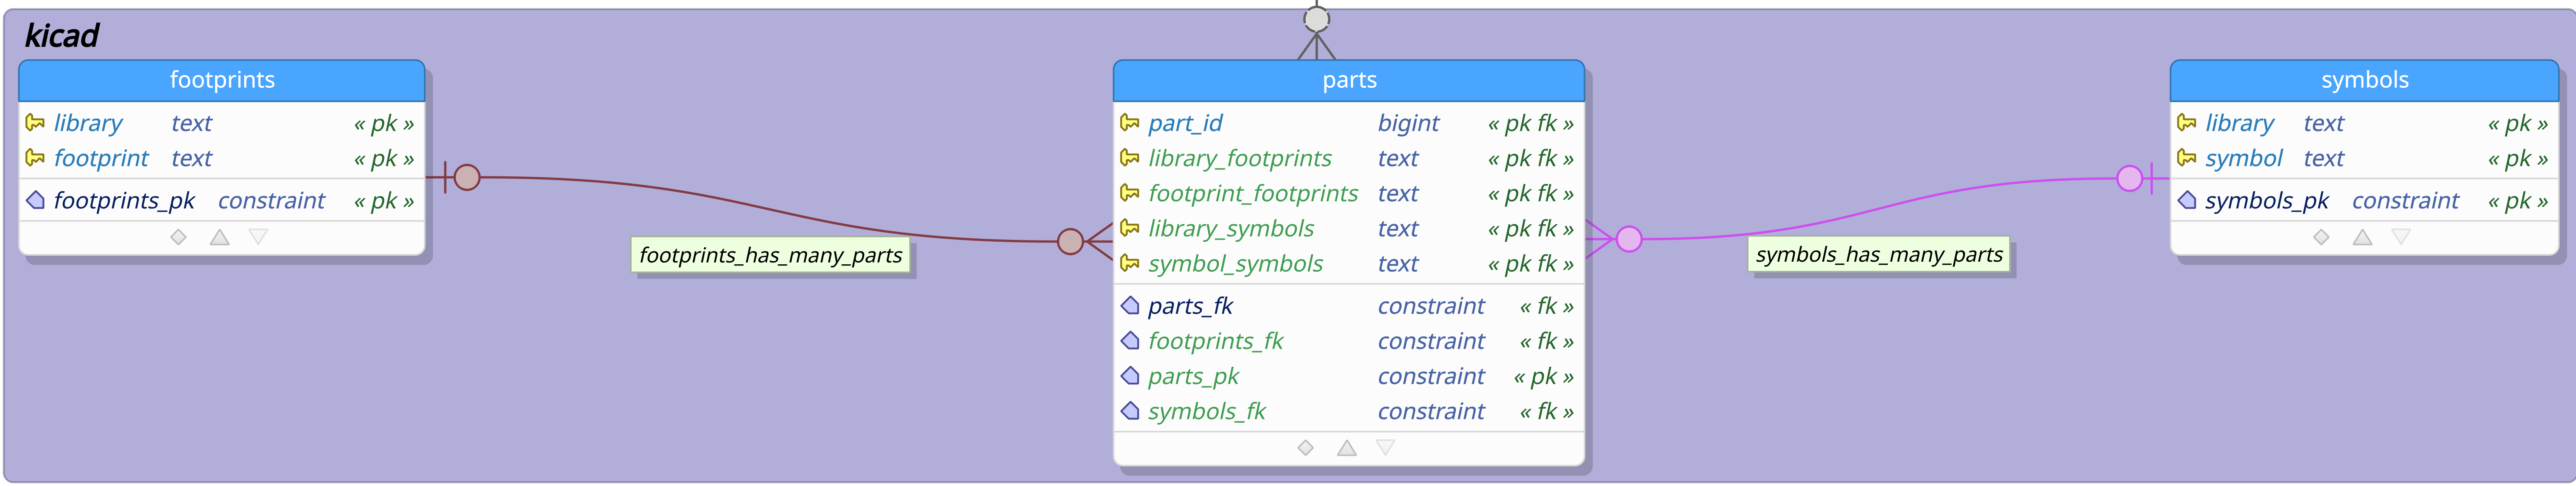
\includegraphics[width=\columnwidth]{db-model_kicad}
	\centering
	\caption{The design of the storage schema}
\end{figure}

\newpage
\subsection{middleware}
The middleware has the task to make the http JSON requests to SQL requesets and than return the data in JSON again.

\newpage
\section{Client}